% Options for packages loaded elsewhere
\PassOptionsToPackage{unicode}{hyperref}
\PassOptionsToPackage{hyphens}{url}
%
\documentclass[
  12pt,
]{article}
\usepackage{lmodern}
\usepackage{amsmath}
\usepackage{ifxetex,ifluatex}
\ifnum 0\ifxetex 1\fi\ifluatex 1\fi=0 % if pdftex
  \usepackage[T1]{fontenc}
  \usepackage[utf8]{inputenc}
  \usepackage{textcomp} % provide euro and other symbols
  \usepackage{amssymb}
\else % if luatex or xetex
  \usepackage{unicode-math}
  \defaultfontfeatures{Scale=MatchLowercase}
  \defaultfontfeatures[\rmfamily]{Ligatures=TeX,Scale=1}
\fi
% Use upquote if available, for straight quotes in verbatim environments
\IfFileExists{upquote.sty}{\usepackage{upquote}}{}
\IfFileExists{microtype.sty}{% use microtype if available
  \usepackage[]{microtype}
  \UseMicrotypeSet[protrusion]{basicmath} % disable protrusion for tt fonts
}{}
\makeatletter
\@ifundefined{KOMAClassName}{% if non-KOMA class
  \IfFileExists{parskip.sty}{%
    \usepackage{parskip}
  }{% else
    \setlength{\parindent}{0pt}
    \setlength{\parskip}{6pt plus 2pt minus 1pt}}
}{% if KOMA class
  \KOMAoptions{parskip=half}}
\makeatother
\usepackage{xcolor}
\IfFileExists{xurl.sty}{\usepackage{xurl}}{} % add URL line breaks if available
\IfFileExists{bookmark.sty}{\usepackage{bookmark}}{\usepackage{hyperref}}
\hypersetup{
  pdftitle={The effect of lexical frequency on word duration: analyzing corpus data in Spanish and English},
  hidelinks,
  pdfcreator={LaTeX via pandoc}}
\urlstyle{same} % disable monospaced font for URLs
\usepackage[margin=1in]{geometry}
\usepackage{graphicx}
\makeatletter
\def\maxwidth{\ifdim\Gin@nat@width>\linewidth\linewidth\else\Gin@nat@width\fi}
\def\maxheight{\ifdim\Gin@nat@height>\textheight\textheight\else\Gin@nat@height\fi}
\makeatother
% Scale images if necessary, so that they will not overflow the page
% margins by default, and it is still possible to overwrite the defaults
% using explicit options in \includegraphics[width, height, ...]{}
\setkeys{Gin}{width=\maxwidth,height=\maxheight,keepaspectratio}
% Set default figure placement to htbp
\makeatletter
\def\fps@figure{htbp}
\makeatother
\setlength{\emergencystretch}{3em} % prevent overfull lines
\providecommand{\tightlist}{%
  \setlength{\itemsep}{0pt}\setlength{\parskip}{0pt}}
\setcounter{secnumdepth}{-\maxdimen} % remove section numbering
\usepackage{tipa}
\usepackage{xcolor}
\usepackage{booktabs}
\usepackage{longtable}
\usepackage{array}
\usepackage{multirow}
\usepackage{wrapfig}
\usepackage{float}
\usepackage{colortbl}
\usepackage{pdflscape}
\usepackage{tabu}
\usepackage{threeparttable}
\usepackage{threeparttablex}
\usepackage[normalem]{ulem}
\usepackage{makecell}
\usepackage{xcolor}
\ifluatex
  \usepackage{selnolig}  % disable illegal ligatures
\fi
\newlength{\cslhangindent}
\setlength{\cslhangindent}{1.5em}
\newlength{\csllabelwidth}
\setlength{\csllabelwidth}{3em}
\newenvironment{CSLReferences}[2] % #1 hanging-ident, #2 entry spacing
 {% don't indent paragraphs
  \setlength{\parindent}{0pt}
  % turn on hanging indent if param 1 is 1
  \ifodd #1 \everypar{\setlength{\hangindent}{\cslhangindent}}\ignorespaces\fi
  % set entry spacing
  \ifnum #2 > 0
  \setlength{\parskip}{#2\baselineskip}
  \fi
 }%
 {}
\usepackage{calc}
\newcommand{\CSLBlock}[1]{#1\hfill\break}
\newcommand{\CSLLeftMargin}[1]{\parbox[t]{\csllabelwidth}{#1}}
\newcommand{\CSLRightInline}[1]{\parbox[t]{\linewidth - \csllabelwidth}{#1}\break}
\newcommand{\CSLIndent}[1]{\hspace{\cslhangindent}#1}

\title{The effect of lexical frequency on word duration: analyzing
corpus data in Spanish and English}
\author{}
\date{\vspace{-2.5em}}

\begin{document}
\maketitle

The present study investigates the effect of lexical frequency on word
duration in Spanish. Previous studies have found that vowel duration in
English is influenced by extra-linguistic factors, such as lexical
frequency (e.g., Gahl, 2008, 2009; Lohman, 2017). The shortening of
frequent forms relative to infrequent ones may correspond to
articulatory routinization, which suggests that neuromotor routines
become more reduced with repetition (Bybee, 2001; Newmeyer, 2006).
However, evidence showing that in homophone pairs (e.g., \emph{thyme} --
\emph{time}), the item with higher frequency is shorter than the
infrequent one reveals that frequency effects on duration may not be due
to repetition of a phonological form but to lemma frequency effects
instead. In the case of Spanish, differences in vowel duration are not
as prominent as in English. Although vowel duration in Spanish
unstressed syllables tends to be shorter than in stressed syllables
(Marín Gálvez, 1994), it is still unclear whether lemma frequency
modulates duration in Spanish.

The present study aims to, first, replicate the frequency effect found
in vowel duration in English (Gahl, 2008; 2009; Lohman, 2017) but in
whole duration. Second, the present study explores the effect of lexical
frequency on word duration in Spanish. This study analyzes English
corpus data from the \emph{Free ST American English Corpus} and Spanish
corpus data from the \emph{Open SLR Corpus}. The English data consisted
of 2806 recordings of cellphone conversations, and the Spanish data
consisted of 1928 recordings of XXX conversations?. Lexical frequency
was measured using the XXX. The data was analyzed using two Bayesian
linear regressions with duration as the outcome variable and speech rate
and orthographic length as fixed predictors.

The results replicated the frequency effects previously found in
English. English frequent words were found to be shorter than infrequent
ones when orthographic length and speech rate were controlled for
(Figure 1). In Spanish, results exhibited a negative linear relationship
between lexical frequency and word duration (Figure 2. Frequent words
were shorter than infrequent ones when orthographic length and speech
rate were controlled for. The findings have implications for
neo-generative (Levelt, 1980), exemplar (Johnson, 1997), and hybrid
(Pierrehumbert, 2016) models of sound representation.

\clearpage

\begin{figure}
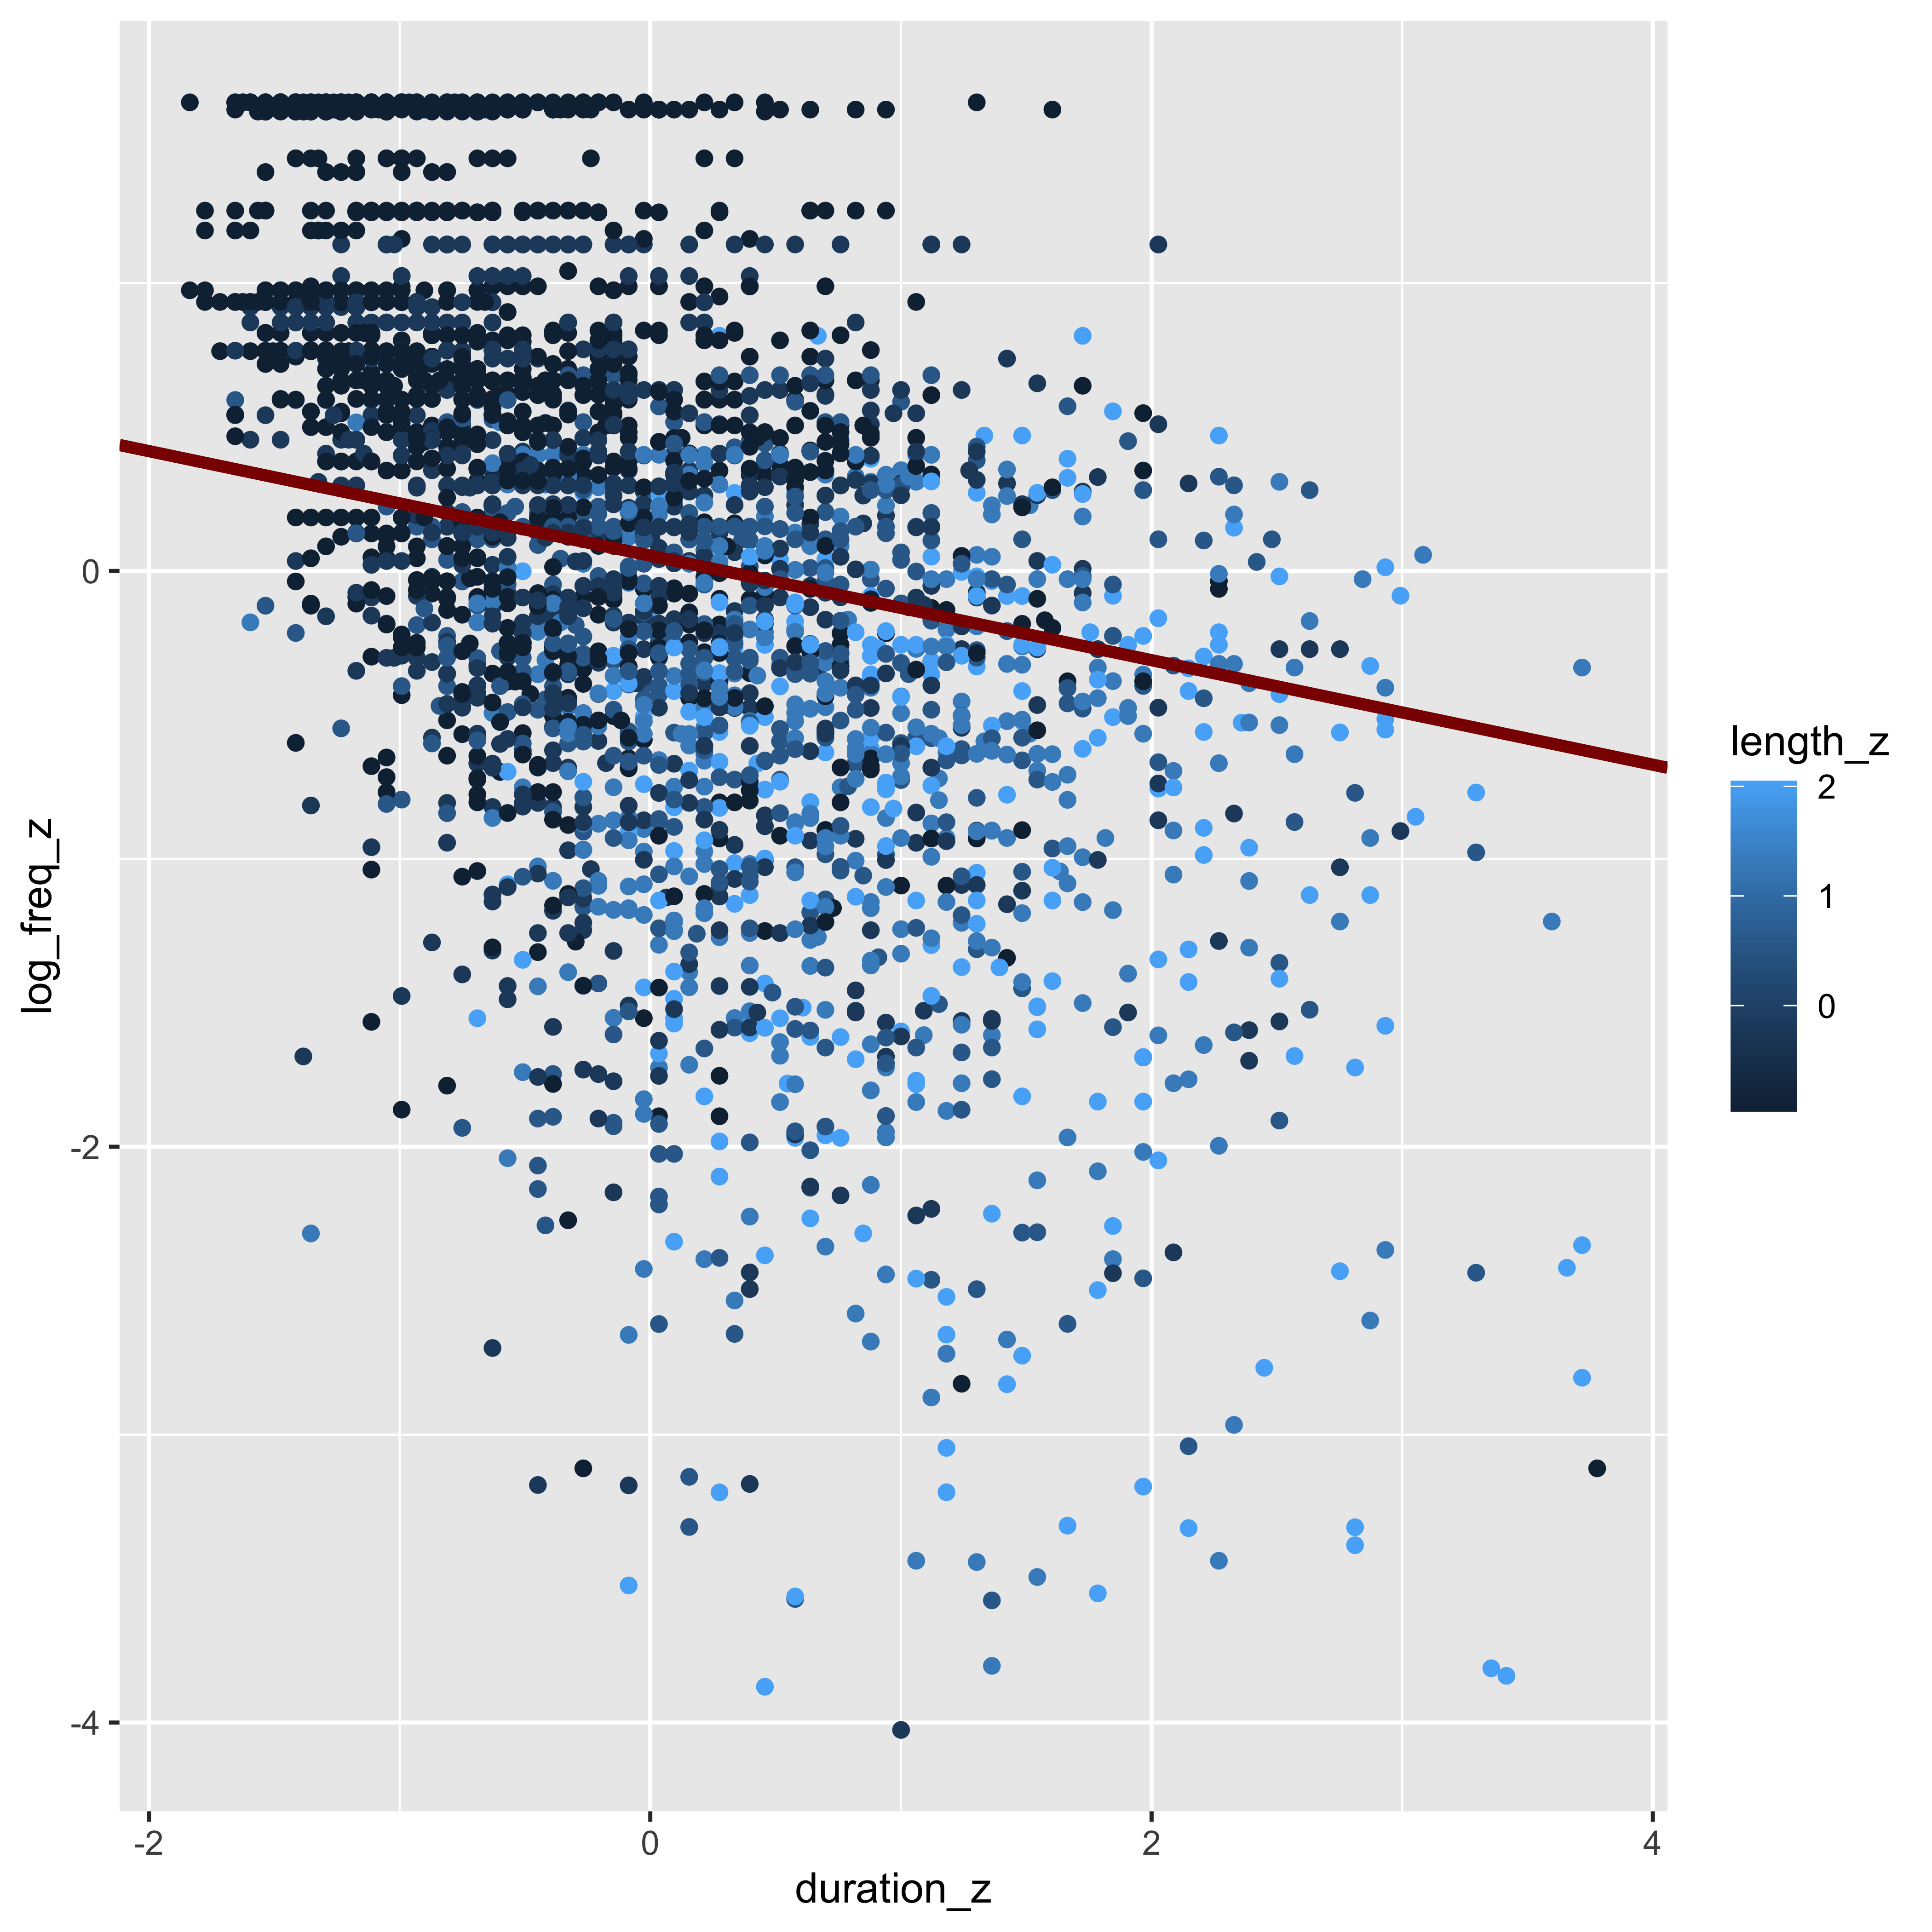
\includegraphics[width=0.5\linewidth]{/Users/juanjogp/Desktop/frequency_duration_spmonolinguals/docs/abstracts/NewSounds22/figs/eng_plot} \caption{Whole word duration in English as a function of lexical frequency with the most plausible line of best fit.}\label{fig:plot-eng}
\end{figure}

\begin{figure}
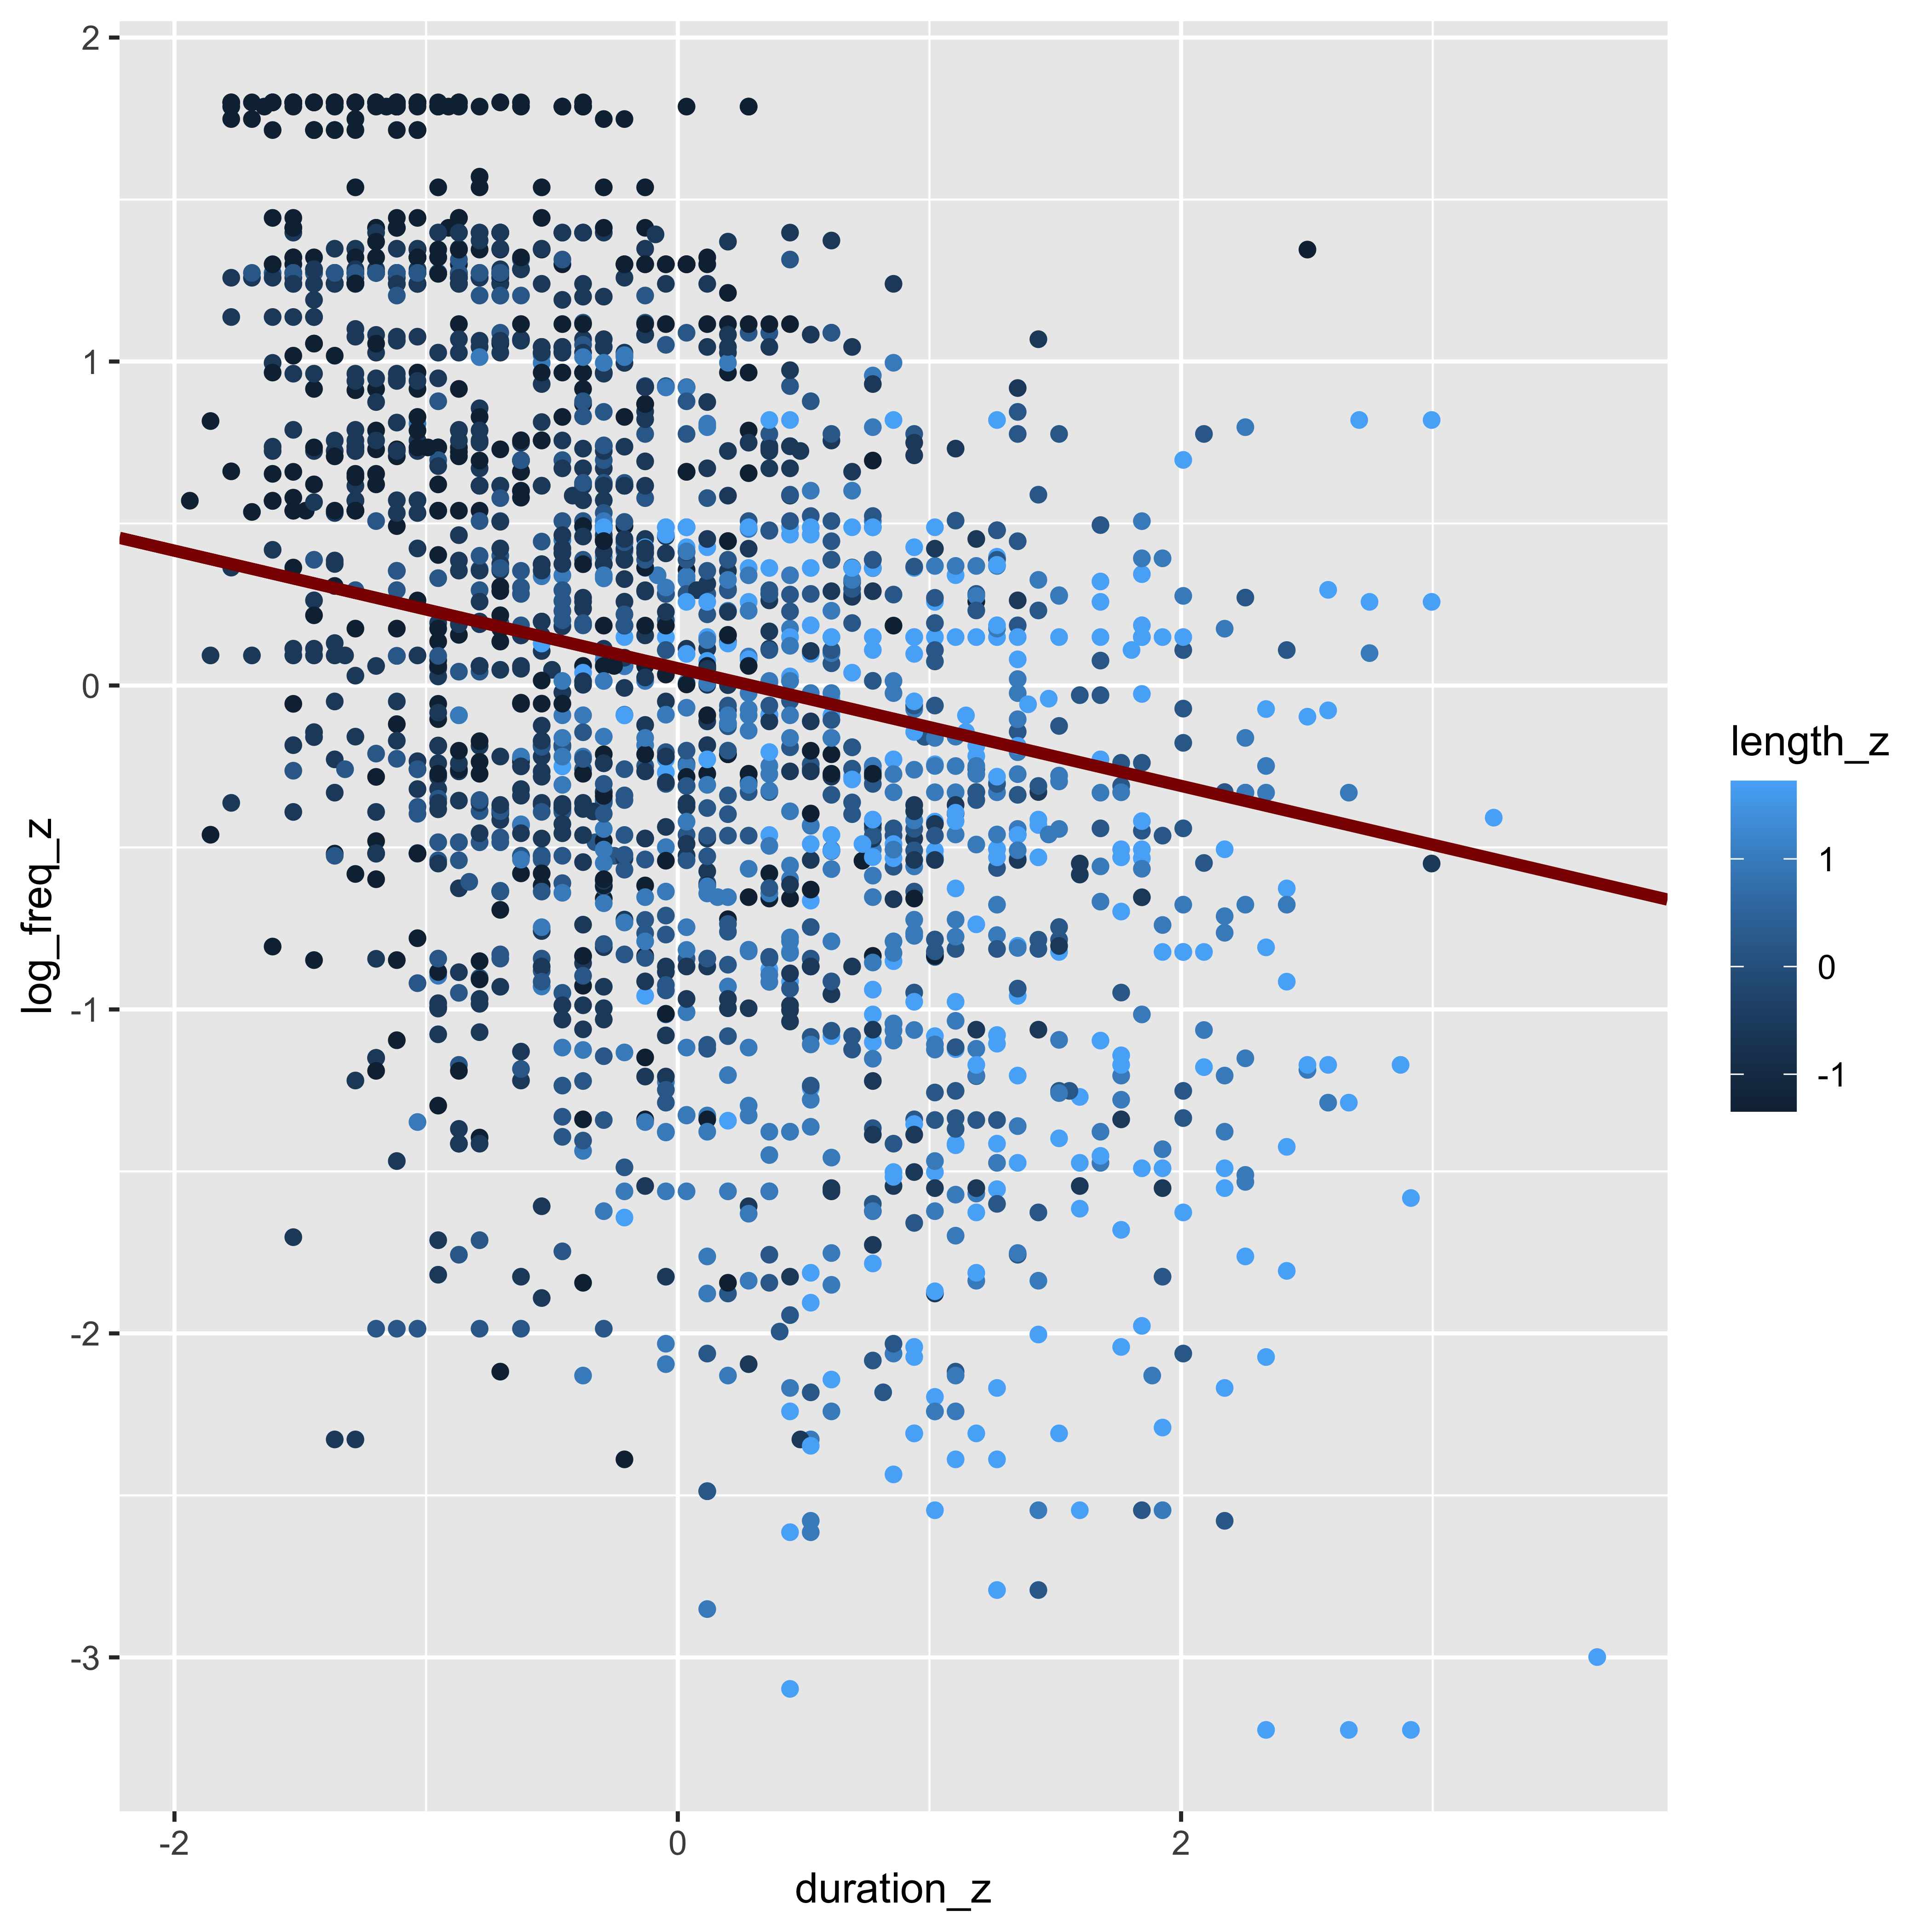
\includegraphics[width=0.5\linewidth]{/Users/juanjogp/Desktop/frequency_duration_spmonolinguals/docs/abstracts/NewSounds22/figs/span_plot} \caption{Whole word duration in Spanish as a function of lexical frequency with the most plausible line of best fit.}\label{fig:plot-span}
\end{figure}

\hypertarget{references}{%
\section{References}\label{references}}

\begingroup
\setlength{\parindent}{-0.5in}
\setlength{\leftskip}{0.5in}

\phantom{.}

\textcolor{white}{\\} \vspace{-0.5in}

\hypertarget{refs}{}
\begin{CSLReferences}{0}{0}
\end{CSLReferences}

\endgroup

\end{document}
